% Five tilings of a strip of length 4 by tiles of length 1 (charcoal) and 2 (rust).
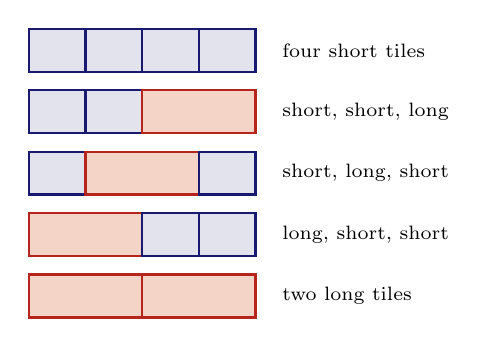
\begin{tikzpicture}[x=0.72cm,y=0.78cm]
  % four short
  \foreach \x in {0,1,2,3} {
    \draw[MidnightBlue,thick,fill=MidnightBlue!12] (\x,4) rectangle (\x+1,4.7);
  }
  \node[font=\scriptsize,anchor=west] at (4.3,4.35) {four short tiles};
  % two short, one long
  \foreach \x in {0,1} {
    \draw[MidnightBlue,thick,fill=MidnightBlue!12] (\x,3) rectangle (\x+1,3.7);
  }
  \draw[BrickRed,thick,fill=BrickRed!15] (2,3) rectangle (4,3.7);
  \node[font=\scriptsize,anchor=west] at (4.3,3.35) {short, short, long};
  % short, long, short
  \draw[MidnightBlue,thick,fill=MidnightBlue!12] (0,2) rectangle (1,2.7);
  \draw[BrickRed,thick,fill=BrickRed!15] (1,2) rectangle (3,2.7);
  \draw[MidnightBlue,thick,fill=MidnightBlue!12] (3,2) rectangle (4,2.7);
  \node[font=\scriptsize,anchor=west] at (4.3,2.35) {short, long, short};
  % long, short, short
  \draw[BrickRed,thick,fill=BrickRed!15] (0,1) rectangle (2,1.7);
  \foreach \x in {2,3} {
    \draw[MidnightBlue,thick,fill=MidnightBlue!12] (\x,1) rectangle (\x+1,1.7);
  }
  \node[font=\scriptsize,anchor=west] at (4.3,1.35) {long, short, short};
  % two long
  \draw[BrickRed,thick,fill=BrickRed!15] (0,0) rectangle (2,0.7);
  \draw[BrickRed,thick,fill=BrickRed!15] (2,0) rectangle (4,0.7);
  \node[font=\scriptsize,anchor=west] at (4.3,0.35) {two long tiles};
\end{tikzpicture}
